\bibliographystyle{babplain-fl}

\chapter{Diseño de Algoritmos}
\label{cha:diseno-de-algoritmos}

  Para demostrar cómo se aplican las técnicas de diseño descritas,
  discutiremos un problema planteado por Bentley~%
    \cite{bentley84:_algorithm_design_techn}.
  Dado el arreglo \(a[n]\), hallar la máxima suma de un rango:
  \begin{equation}
    \label{eq:problema}
    \max_{i, j} \left\{ \sum_{i \le k \le j} a[k] \right\}
  \end{equation}
  Si todos los valores son positivos,
  la respuesta es obvia:
  la suma de todos los elementos del arreglo.
  El punto está si hay elementos negativos:
  ¿incluimos uno de ellos
  en la esperanza que los elementos positivos que lo rodean
  más que lo compensen?
  Finalmente,
  acordamos que la suma de un rango vacío es cero,
  y que en un arreglo de elementos negativos la suma máxima es cero.

\section{Algoritmo ingenuo}
\label{sec:algoritmo-1}

  La solución obvia,
  traducción directa de la especificación
  dada por la ecuación~\eqref{eq:problema},
  es la mostrada en el programa C del listado~\ref{lst:algoritmo-1}.
  \lstinputlisting[float,
                   language = C,
                   firstline = 8,
                   caption = {Algoritmo 1: Versión ingenua},
                   label = lst:algoritmo-1]
                  {code/max-sum-1.c}
  La complejidad del algoritmo~1 es \(O(n^3)\).
  Lo que buscamos es mejorarlo.

\section{No recalcular sumas}
\label{sec:no-recalcular-sumas}

  Hay dos ideas sencillas para evitar recalcular sumas.

\subsection{Extender sumas}
\label{sec:algoritmo-2}

  En vez de calcular la suma del rango cada vez,
  extendemos la suma anterior.
  Esto da el programa del listado~\ref{lst:algoritmo-2}.
  \lstinputlisting[float,
                   language = C,
                   firstline = 8,
                   caption = {Algoritmo 2: Evitar recalcular sumas},
                   label = lst:algoritmo-2]
                  {code/max-sum-2.c}
  La complejidad del algoritmo~2 es \(O(n^2)\).

\subsection{Sumas cumulativas}
\label{sec:algoritmo-3}

  Una manera de manejar rangos es usar sumas cumulativas,
  y obtener el valor para el rango restando.
  Esta idea da el listado~\ref{lst:algoritmo-3}.
  \lstinputlisting[float,
                   language = C,
                   firstline = 8,
                   caption = {Algoritmo 3: Usar arreglo cumulativo},
                   label = lst:algoritmo-3]
                  {code/max-sum-3.c}
  La complejidad del algoritmo~3 es \(O(n^2)\).
  Comparado a nuestro algoritmo original resulta una mejora,
  pero no respecto a la segunda variante.

\section{Dividir y Conquistar}
\label{sec:algoritmo-4}

  Aplicar la estrategia discutida en el capítulo~\ref{cha:dividir-conquistar}
  lleva a la figura~\ref{subfig:Algoritmo-4-AB}.
  Pero debemos también considerar que el rango con máxima suma
  esté a horcajadas,
  cruzando el punto central,
  como en la figura~\ref{subfig:Algoritmo-4-C}.
  \begin{figure}[ht]
    \centering
    \subfloat[Máximos en las mitades]{
      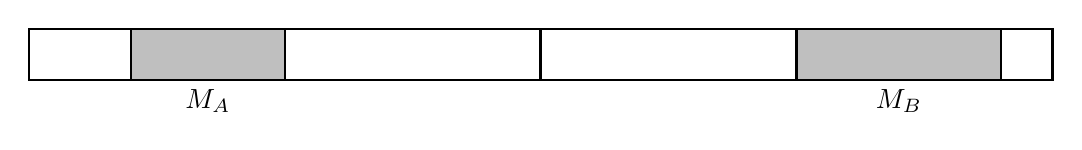
\begin{tikzpicture}[scale = 0.65]
        \draw[thick] (0, 0) rectangle (20, 1);
        \draw[thick] (10, 0) -- (10, 1);

        \draw[fill = lightgray, thick] (2, 0) rectangle (5, 1);
        \node at (3.5, 0) [below] {\(M_A\)};

        \draw[fill = lightgray, thick] (15, 0) rectangle (19, 1);
        \node at (17, 0) [below] {\(M_B\)};
      \end{tikzpicture}
      \label{subfig:Algoritmo-4-AB}
    } \\
    \subfloat[Máximo al medio]{
      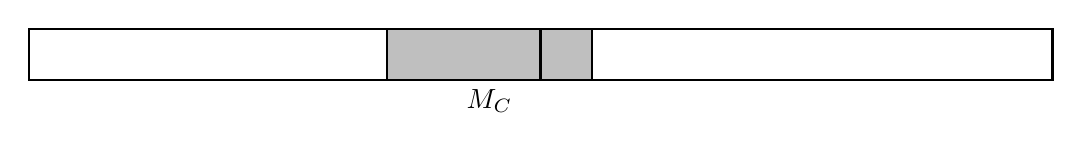
\begin{tikzpicture}[scale = 0.65]
        \draw[fill = lightgray, thick] (7, 0) rectangle (11, 1);
        \draw[thick] (0, 0) rectangle (20, 1);
        \draw[thick] (10, 0) -- (10, 1);

        \node at (9, 0) [below] {\(M_C\)};
      \end{tikzpicture}
      \label{subfig:Algoritmo-4-C}
    }
    \caption{Dividir y conquistar}
    \label{fig:algoritmo-4}
  \end{figure}
  El algoritmo es el dado en el listado~\ref{lst:algoritmo-4}.
  \lstinputlisting[float,
                   language = C,
                   firstline = 8,
                   caption = {Algoritmo 4: Dividir y conquistar},
                   label = lst:algoritmo-4]
                  {code/max-sum-4.c}
  Usando el teorema maestro
  (teorema~\ref{theo:master-theorem}),
  para el algoritmo~4 son \(a = 2\), \(b = 2\) y  \(f(n) = O(n)\),
  por lo tanto la complejidad es \(O(n \log n)\).

\section{Un algoritmo lineal}
\label{sec:algoritmo-5}

  Otro algoritmo resulta de la idea,
  común al procesar arreglos,
  de tener una solución parcial hasta \(a[i]\),
  y analizar cómo extenderla para cubrir hasta \(a[i + 1]\).
  En nuestro caso,
  esto significa considerar la máxima suma que llega hasta \(a[i]\),
  y recordar la máxima suma vista hasta ahora,
  ver la figura~\ref{fig:Algoritmo-5}.
  Gries~%
    \cite{gries82:_note_strategy_loop_inv}
  deriva el algoritmo sistemáticamente
  y demuestra su correctitud.
  Esto da el algoritmo~5,
  del listado~\ref{lst:algoritmo-5}
  \begin{figure}[ht]
    \centering
    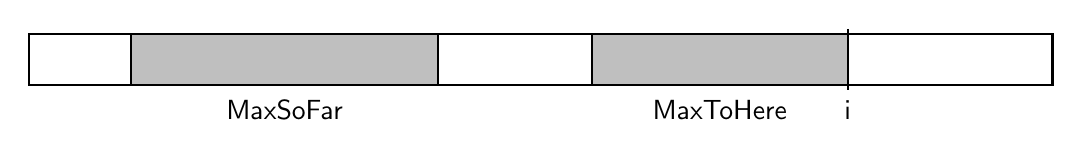
\begin{tikzpicture}[scale = 0.65]
      \draw[thick] (0, 0) rectangle (20, 1);

      \draw[fill = lightgray, thick] (2, 0) rectangle (8, 1);
      \node at (5, -0.1) [below] {\textsf{MaxSoFar}};

      \draw[fill = lightgray, thick] (11, 0) rectangle (16, 1);
      \node at (13.5, -0.1) [below] {\textsf{MaxToHere}};

      \draw[thick] (16, 1.1) -- (16, -0.1) node [below] {\textsf{i}};
    \end{tikzpicture}
    \caption{Extender la solución}
    \label{fig:Algoritmo-5}
  \end{figure}

  \lstinputlisting[float,
                   language = C,
                   firstline = 8,
                   caption = {Algoritmo 5: Ir extendiendo resultado parcial},
                   label = lst:algoritmo-5]
                  {code/max-sum-5.c}
  La complejidad del algoritmo~5 es \(O(n)\).
  Claramente es imposible tener una complejidad menor que \(n\),
  dado que es necesario revisar cada elemento del arreglo.

  \begin{table}[ht]
    \centering
    \begin{tabular}{r|*{5}{|c}}
      \multicolumn{1}{c||}{\textbf{Algoritmo}}
         & \textbf{1} & \textbf{2} & \textbf{4} & \textbf{5} \\
      \hline
      \multicolumn{1}{l||}{Líneas de C} & 8 & 7 & 14 & 7 \\
      \hline
      \multicolumn{1}{l||}{Tiempo en \([\mu \mathrm{s}]\)}
            & \(3.4 n^3\) & \(13 n^2\) & \(46 n \log n\) & \(33 n\) \\
      \hline
      Tiempo para \(n = {}\)
        \(10^2\) & \(3.4 [\mathrm{s}]\)	 & \(130 [\mathrm{ms}]\)
                 & \(30 [\mathrm{ms}]\)	 & \(3,3 [\mathrm{ms}]\) \\
        \(10^3\) & \(0,94 [\mathrm{h}]\) & \(14 [\mathrm{s}]\)
                 & \(0,45 [\mathrm{s}]\) & \(33 [\mathrm{ms}]\) \\
        \(10^4\) & \(39 \text{ días}\)	 & \(22 [\mathrm{min}]\)
                 & \(6,1 [\mathrm{s}]\)	 & \(0.33 [\mathrm{s}]\) \\
        \(10^5\) & \(108 \text{ años}\)	 & \(1,5 \text{ días}\)
                 & \(1,3[\mathrm{min}]\) & \(3,3 [\mathrm{s}]\) \\
        \(10^6\) & \(108 \text{ millones de años}\) & \(5 \text{ meses}\)
                 & \(15 [\mathrm{min}]\) & \(33 [\mathrm{s}]\)
    \end{tabular}
    \caption{Comparativa de Bentley~%
               \cite{bentley84:_algorithm_design_techn}
             entre las variantes}
    \label{tab:comparativa-algoritmos}
  \end{table}
  Reportar la complejidad de un algoritmo en términos de \(O(\cdot)\)
  es incompleto,
  pero el cuadro~\ref{tab:comparativa-algoritmos} muestra su relevancia.
  La ventaja es que la complejidad en estos términos es sencilla de obtener,
  en nuestros casos simples
  (algoritmos 1, 2, 3 y 5)
  por inspección,
  el teorema maestro da la complejidad para el algoritmo 4 directamente.

\section{Mayoría de una secuencia}
\label{sec:mayoria-secuencia}

  Se dice que un elemento de una secuencia de \(n\) elementos
  es \emph{mayoría} si es más de \(\lfloor n / 2 \rfloor\) elementos de ella.
  Nuestro problema es,
  dada una secuencia que sabemos tiene una mayoría,
  determinar cuál es ese elemento.

  Algoritmos obvios para resolver este problema son ordenar la secuencia
  y ver el elemento del medio
  (es claro que si cierto elemento
   es al menos la mitad de la secuencia ordenada,
   estará al medio,
   independiente de dónde comience la repetición).
  Esto lo podemos mejorar viendo que solo interesa el elemento del medio,
  basta determinar la mediana.
  O podemos ir contabilizando repeticiones de cada elemento,
  almacenándolos por ejemplo en un árbol
  o una tabla \emph{\foreignlanguage{english}{hash}}.

  La primera idea demora \(O(n \log n)\),
  y exige tener la secuencia completa a la mano.
  Es posible determinar la mediana en tiempo \(O(n)\),
  pero los algoritmos con engorrosos.
  La tercera puede procesar la secuencia conforme llega,
  usando tablas \emph{\foreignlanguage{english}{hash}},
  demora \(O(n)\) en promedio,
  pero requiere \(O(n)\) espacio adicional.

  Boyer y Moore~%
    \cite{boyer91:_mjrty_fast_majority_vote_algor}
  propusieron un algoritmo que lee la secuencia una sola vez
  y usa una cantidad mínima de espacio adicional.
  El algoritmo es el~\ref{alg:MJRTY}.
  \begin{algorithm}[ht]
    \DontPrintSemicolon\Indp

    \Function{\(mathrm{MJRTY}(S)\)}{
      \(\mathrm{count} \gets 0\) \;
      \ForEach{\(x \in S\)}{
        \uIf{\(\mathrm{count} = 0\)}{
          \(m \gets x\) \;
          \(\mathrm{count} \gets 1\) \;
        }
        \uElseIf{\(m = x\)}{
          \(\mathrm{count} \gets \mathrm{count} + 1\) \;
        }
        \Else{
          \(\mathrm{count} \gets \mathrm{count} - 1\) \;
        }
        \Return \(m\) \;
      }
    }
    \caption{Algoritmo MJRTY de Boyer-Moore}
    \label{alg:MJRTY}
  \end{algorithm}
  La idea es ir contabilizando elementos iguales al candidato a mayoría,
  si aparecen más elementos diferentes que iguales a la mayoría propuesta,
  cambiamos de candidato.

  La demostración de que el misterioso algoritmo~\ref{alg:MJRTY} es correcto
  es como sigue:
  sea \(c\) una variable fantasma cuyo valor es el de \(\mathrm{count}\)
  si \(m\) es la mayoría,
  \(- \mathrm{count}\) en caso contrario.
  Cada vez que el algoritmo se encuentra con un valor igual a la mayoría,
  \(c\) aumenta
  (si \(m\) es la mayoría,
   aumenta \(\mathrm{count}\) en uno;
   si no es la mayoría,
   \(\mathrm{count}\) disminuye en uno);
  cada vez que encuentra un valor diferente a la mayoría,
  \(c\) puede aumentar o disminuir en uno.
  Habrán más aumentos que disminuciones de \(c\),
  con lo que \(c\) al final del algoritmo es positivo.
  Pero esto solo es posible si \(\mathrm{count}\) es positivo,
  y esto a su vez es solo si \(m\) es la mayoría.

  Está claro que este algoritmo siempre retorna un valor,
  no detecta si la secuencia no tiene mayoría.
  Verificar esto requiere una segunda pasada por la secuencia.

\bibliography{../referencias}

%%% Local Variables:
%%% mode: latex
%%% TeX-master: "../INF-221_notas"
%%% ispell-local-dictionary: "spanish"
%%% End:

% LocalWords:  eq cumulativas correctitud english hash MJRTY
